% Numerical Results ----------------------------------------------------------------------------------------------------------------------------------------------------------------
\section{Numerical Results}
\subsection{Rate of Convergence}
\label{subsec:conv_rate_ell}
To replicate the theoretical rate of convergence we first consider a sequence of uniform meshes. 
Let $h_l = 2^{-l}$ denote the global (uniform) meshsize and $\mathcal{T}_h^{(l)}$ denote
the partitions of $\Omega$ for $l = 2,\ldots,9$. As an example we have $\mathcal{T}_h^{(2)} = \{(0, 0.25), (0.25, 0.5),(0.5, 0.75),(0.75, 1)\}$. 
To begin we worked with the constant coefficient $c\equiv 1$. In this case choosing $\sigma = 10(r+1)^2$ was more than enough to guarantee positive definiteness of the 
system matrix.
We tested our methods programmed in \texttt{MATLAB} using some very simple exact solutions $u \in C^1(\Omega)$, approximated them numerically finding some $u_h \in V_h^r(\mathcal{T}_h^{(l)})$ 
(for an a priori fixed polynomial degree $r$) and calculated the $L^2$-norm
\begin{equation}
	\|u - u_h\|_{L^2(\Omega)} = \Big( \int_{\Omega} |u(x) - u_h(x)|^2 \text{d} x \Big)^{1/2} = \Big( \sum_{n=0}^{N_l}\int_{I_n} |u(x) - u_h(x)|^2 \text{d} x \Big)^{1/2} \nonumber
\end{equation}
and the broken $H^1$-norm

\begin{equation}
	\|u - u_h\|_{H^1(\mathcal{T}_h^{(l)} )} = \Big( \sum_{n=0}^{N_l}\int_{I_n} |u^{\prime}(x) - u_h^{\prime}(x)|^2 \text{d} x \Big)^{1/2}. \nonumber
\end{equation}
Note that even though $u_h$ is not in $H^1(\Omega)$ and we can therefore not calculate the normal $H^1$-norm, we do have 

\begin{equation}
	u, u_h \in H^1(\mathcal{T}_h^{(l)}) = \{v \in L^2(\Omega) | v|_{I_n} \in  H^1(I_n) \text{ for } n = 0,\ldots,N_l\} \nonumber
\end{equation}
so taking the broken Sobolev norm makes sense also for $V_h$ functions.

Firstly to ensure the exactness of the method we chose
the exact solution $u(x) = x^r$ and approximated it using $\mathcal{P}^r$ elements. As expected we got a minimal floating-point error of around $10^{-15}$
in both $L^2$-, and $H^1(\mathcal{T}^{(l)}_h)$-norms, slightly increasing for increasing $l$ due to the growing condition number of the system matrix.
This indicates exactness of the method.

Next we considered the exact solution $u(x) = e^{-x} \sin(x)$, we observed the with the theory conforming convergence rates 
$\mathcal{O}(h^r), \mathcal{O}(h^{r+1})$, in the $H^1(\mathcal{T}_h)$- and $L^2$-norm respectively for $\mathcal{P}^r$-elements. As visible in figures 
\ref{fig:elliptic_uniform_mesh_error_p1}, \ref{fig:elliptic_uniform_mesh_error_p2}

\begin{figure}[h!]
    \centering
    
    \begin{minipage}[t]{0.48\textwidth}
        \centering
        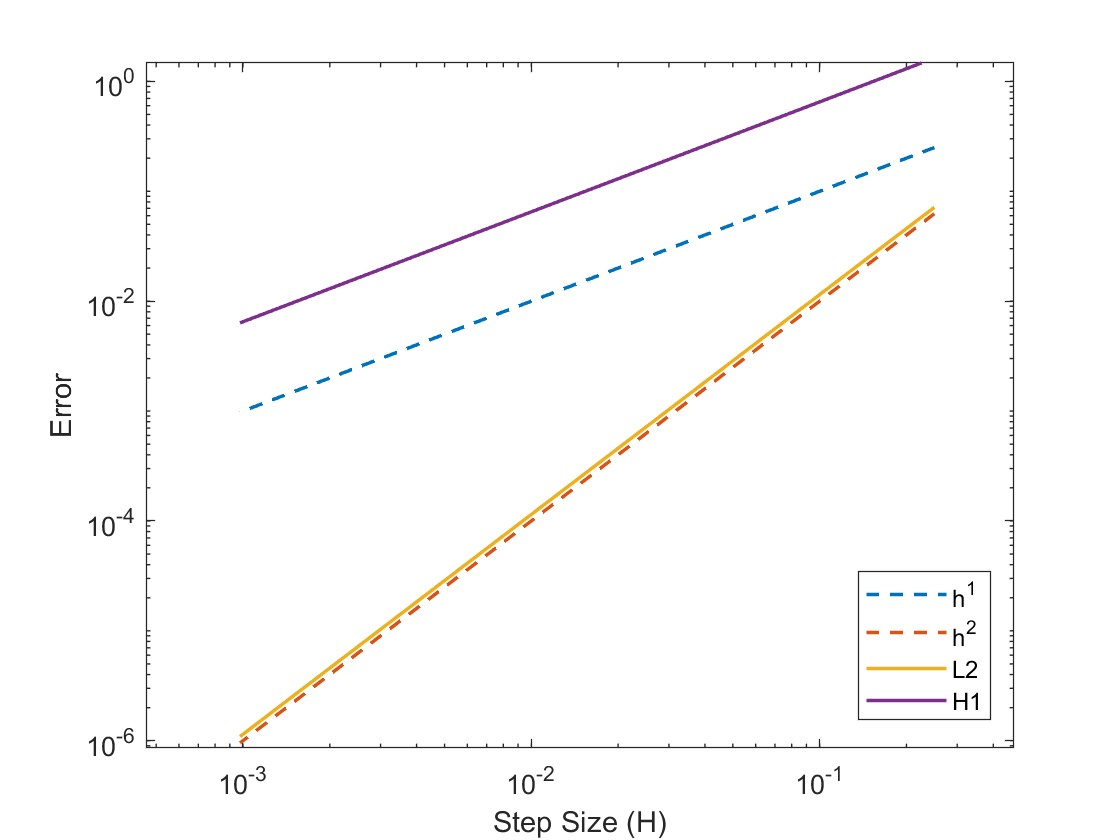
\includegraphics[width=\linewidth]{figures/dg_elliptic_uniform_mesh_exact_sol_errors_P1.jpg}
        \caption{Errors of SIPG for $P^1$-elements}
        \label{fig:elliptic_uniform_mesh_error_p1}
    \end{minipage}
    \hfill
    \begin{minipage}[t]{0.48\textwidth}
        \centering
        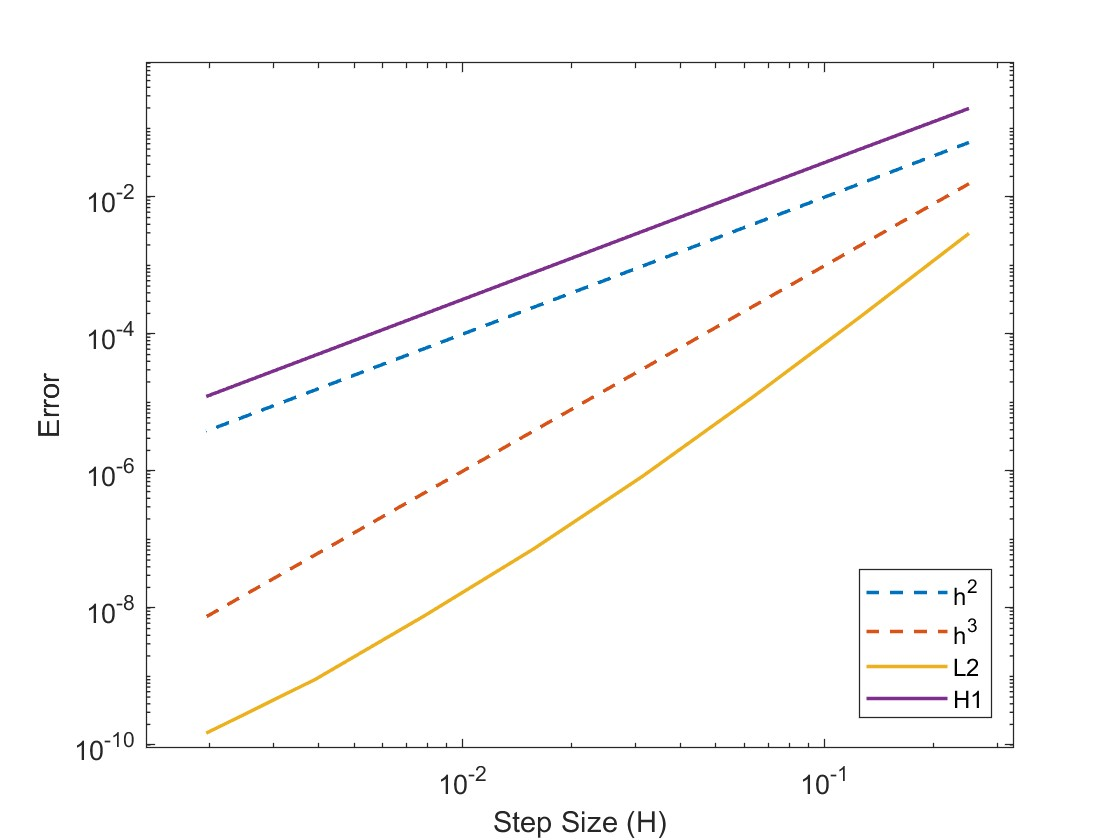
\includegraphics[width=\linewidth]{figures/dg_elliptic_uniform_mesh_exact_sol_errors_P2.jpg}
        \caption{Errors of SIPG for $P^2$-elements}
        \label{fig:elliptic_uniform_mesh_error_p2}
    \end{minipage}
\end{figure}

We plotted the numerical solution for $\mathcal{P}^1, \mathcal{P}^2$-elements in the figures 
\ref{fig:elliptic_uniform_mesh_sol_p1}, \ref{fig:elliptic_uniform_mesh_sol_p2} respectively on the partition $\mathcal{T}_h^{(3)}$, i.e. for 
8 elements with meshsize $h = \frac{1}{8}$. By eye the solution seems continuous, this is due to the high penalization parameter 
$\sigma = 10(r+1)^2$. In fact the solution is not continuous and the boundary conditions are not exact either, the error is just not noticeable
by eye. 

\begin{figure}[h!]
    \centering
    
    \begin{minipage}[t]{0.48\textwidth}
        \centering
        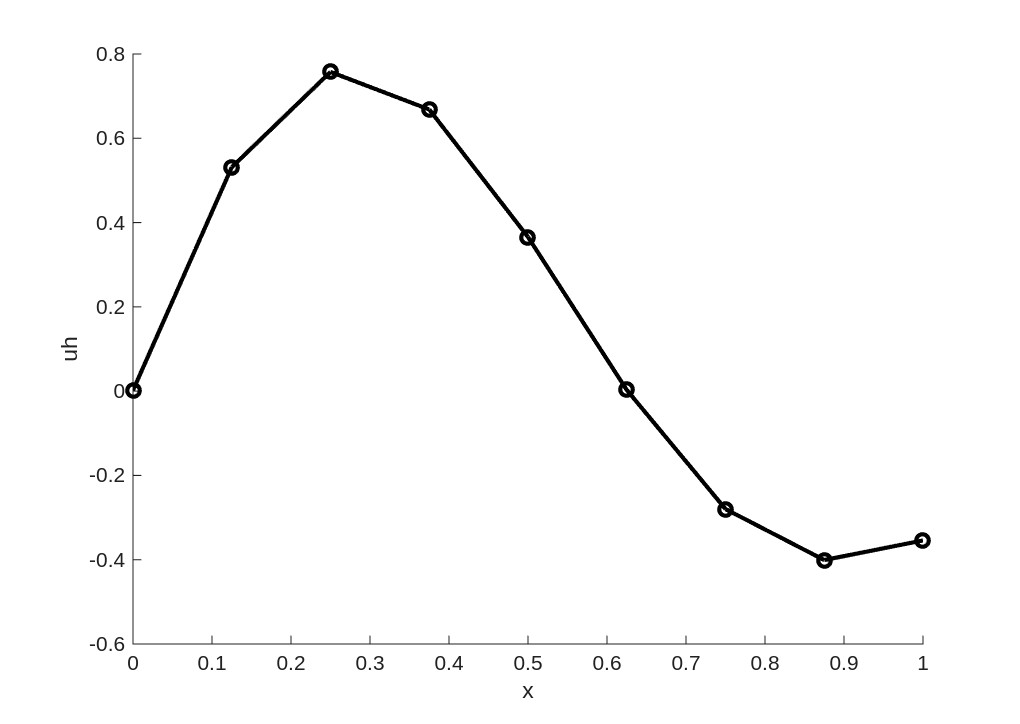
\includegraphics[width=\linewidth]{figures/dg_elliptic_num_sol_p1.jpg}
        \caption{numerical SIPG-approximation for $P^1$-elements}
        \label{fig:elliptic_uniform_mesh_sol_p1}
    \end{minipage}
    \hfill
    \begin{minipage}[t]{0.48\textwidth}
        \centering
        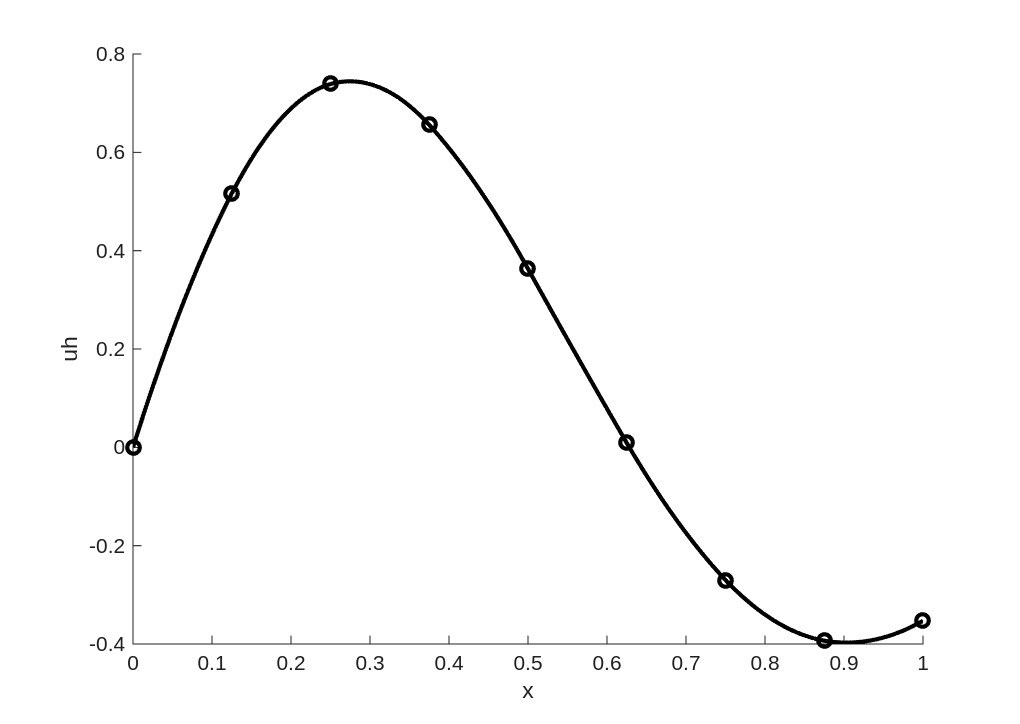
\includegraphics[width=\linewidth]{figures/dg_elliptic_num_sol_p2.jpg}
        \caption{numerical SIPG-approximation for $P^2$-elements}
        \label{fig:elliptic_uniform_mesh_sol_p2}
    \end{minipage}
\end{figure}

If we reduce the penalization parameter enough such that the bilinear form 
is no longer coercive we can observe the jumps growing and the discontinuity becomes apparent as is visible in figures 
\ref{fig:elliptic_uniform_mesh_sol_p1_non_coercive}, \ref{fig:elliptic_uniform_mesh_sol_p2_non_coercive} where we have set $\sigma = 1.1$. 
Maybe interesting to observe is the effect of enforcing boundary conditions weakly. Clearly here the Dirichlet boundary condition $u(0) = 0$ is 
not fulfilled by the numerical solutions, which would be the case for strongly enforced boundary conditions. \\

\begin{figure}[h!]
    \centering
    
    \begin{minipage}[t]{0.48\textwidth}
        \centering
        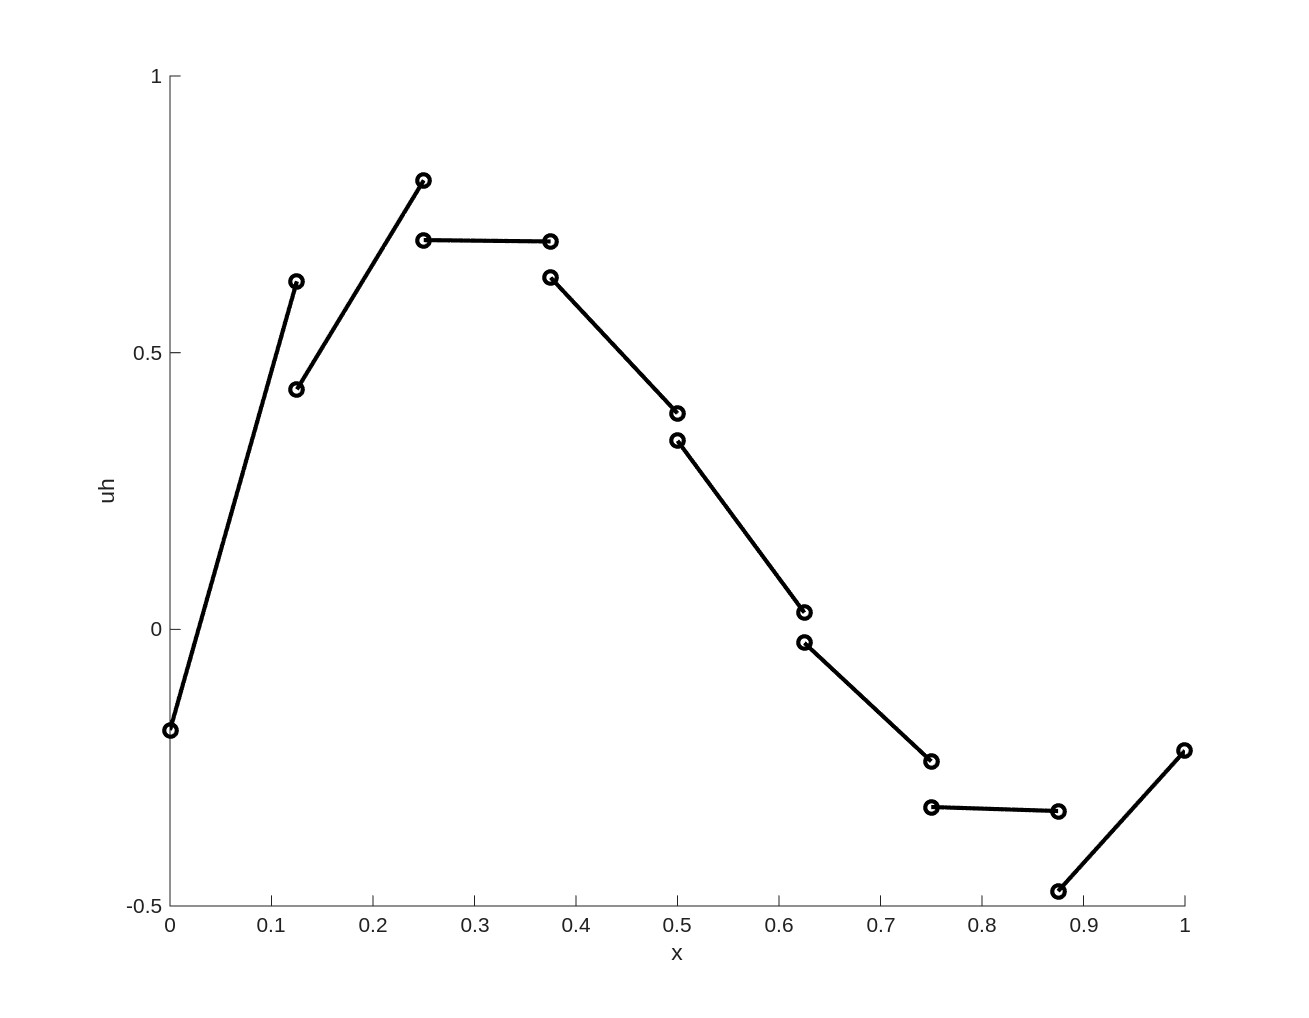
\includegraphics[width=\linewidth]{figures/dg_elliptic_num_sol_non_coercive_p1.jpg}
        \caption{numerical SIPG-approximation for $P^1$-elements with small penalty}
        \label{fig:elliptic_uniform_mesh_sol_p1_non_coercive}
    \end{minipage}
    \hfill
    \begin{minipage}[t]{0.48\textwidth}
        \centering
        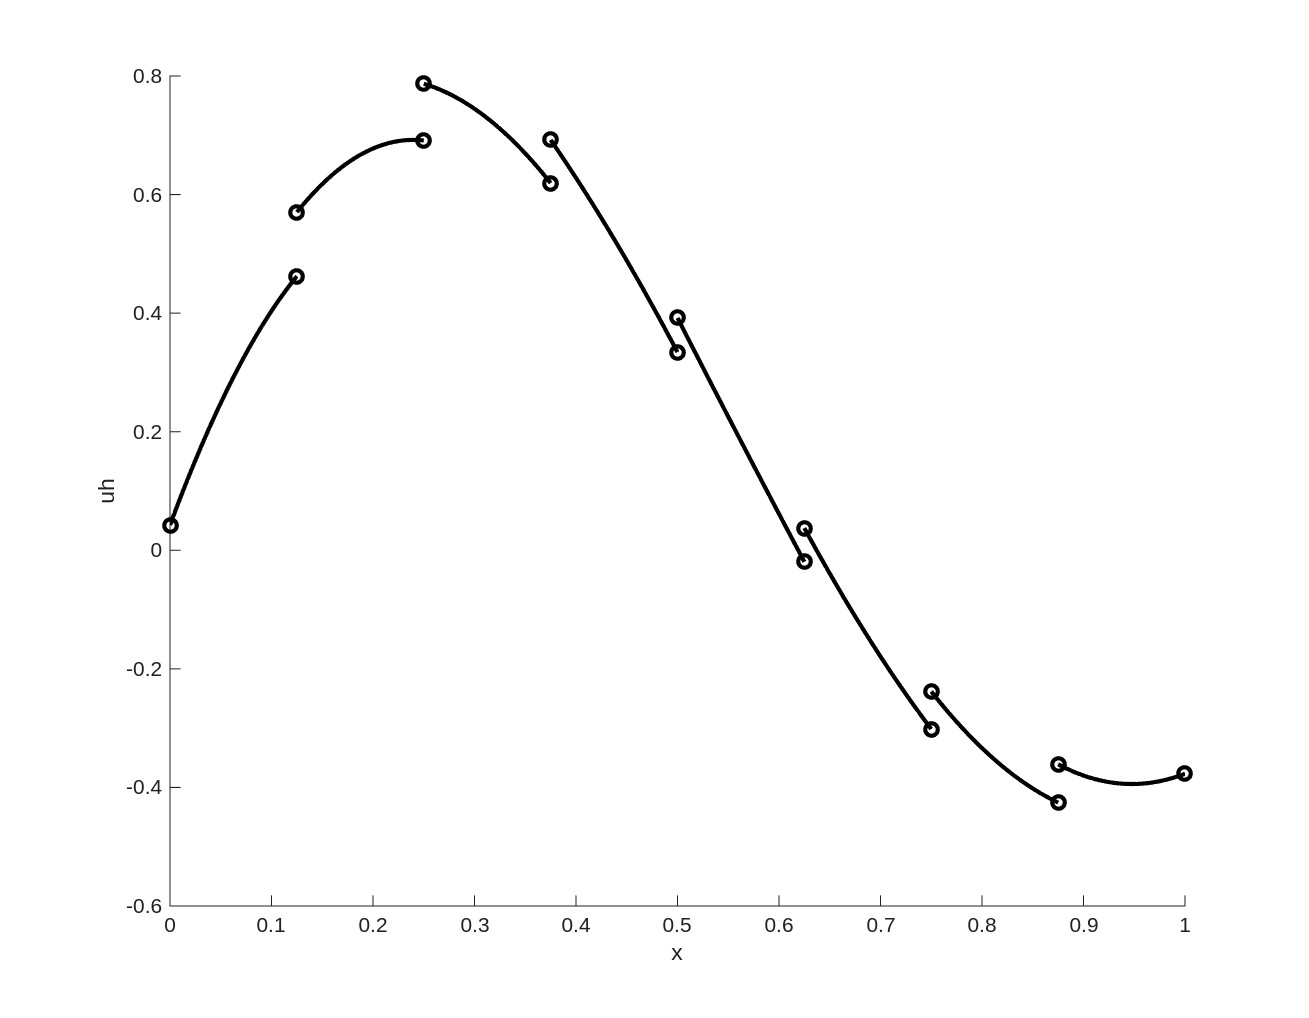
\includegraphics[width=\linewidth]{figures/dg_elliptic_num_sol_non_coercive_p2.jpg}
        \caption{numerical SIPG-approximation for $P^2$-elements with small penalty}
        \label{fig:elliptic_uniform_mesh_sol_p2_non_coercive}
    \end{minipage}
\end{figure}

Finally we repeated the tests above using a non constant yet still smooth coefficient $c(x) = \sin(10x) + 2$. We observed the same convergence rates but slightly higher
errors overall. This was to be expected since for a non-constant $c$ we introduce a quadrature error. 

\subsection{Influence of Quadrature Rule on the Convergence Rate}
As noted in section \ref{sec:ell_basis} by using $r+1$ Gauss-Lobatto nodes (in the context of $\mathcal{P}^r$-elements) as quadrature nodes and basis nodes at the same time
introduces an error when assembling the mass matrix of the system. In this subsection we experimentally compare the results of using $r+1$ Gauss-Lobatto quadrature nodes
to approximate the integrals versus using the exact integration values. To be precise we fix a polynomial degree $r$ and our Lagrangian basis with $r+1$ Gauss-Lobatto nodes
as specified in section \ref{sec:ell_basis} and approximate all integrals first using the Gauss-Lobatto quadrature rule with $r+1$ nodes, then with $r+2$ nodes and compare the two.
\\
First we have to consider a slightly different elliptical problem, which requires a mass matrix. 
\begin{equation}
	\label{eq:elliptic_pde}
	-(c(x)u'(x))' + u(x) = f(x) \qquad \forall x\in \Omega \nonumber
\end{equation}
\begin{equation}
	\label{eq:elliptic_pde_bc}
	u(0) = g_0, u(1) = g_1 \nonumber
\end{equation}
We can apply the exact same tools as in the derivation of the variational formulation in section \ref{sec:elliptic_var_form} and get the discrete SIPG variational formulation. \\
Find $u_h \in V_h$ such that:
\begin{equation}
	\label{eq:discrete_var_form_elliptic_with_mass}
	b_h(u_h, v) + (u_h, v)_{L^2(\Omega)} = \ell_h(v), \qquad \forall v\in V_h 
\end{equation}
Now analogously to section \ref{sec:matrix_vect_syst} we write $u_h = \sum_{m=0}^{N} \sum_{j=0}^r \alpha_j^m \Phi_j^m \in V_h$ and find that (\ref{eq:discrete_var_form_elliptic_with_mass})
is equivalent to \\
\begin{equation*}
	\sum_{m=0}^{N} \sum_{j=0}^r \alpha_j^m \Big(b_h(\Phi_j^m, \Phi_i^n) + (\Phi_j^m, \Phi_i^n)_{L^2(\Omega)}\Big) = \ell_h(\Phi_i^n) \qquad \forall i \in \{0,\ldots,r\}, \{n = 0,\ldots,N\}
\end{equation*}
which in turn is equivalent to the Matrix-Vector system

\begin{equation}
	\label{eq:elliptic_matrix_vect_system_with_mass}
	\Big( \textbf{B} + \textbf{M} \Big) \textbf{u} = \textbf{l}
\end{equation}
where as before 
$ [\textbf{B}]_{T(n,i), T(m,j)} = b_h(\Phi_j^m, \Phi_i^n),
	[\textbf{u}]_{T(m,j)} = \alpha_j^m,
	[\textbf{l}]_{T(n,i)} = \ell_h(\Phi_i^n)$ and furthermore
$ [\textbf{M}]_{T(n,i), T(m,j)} = (\Phi_j^m, \Phi_i^n)_{L^2(\Omega)}$.
\\ \\
Next we considered the same setting as described in subsection \ref{subsec:conv_rate_ell} and tested the convergence rates for $\mathcal{P}^1,\mathcal{P}^2$-elements,
where we chose the exact solution $u(x) = e^{-x}\sin(x)$ and $c(x) = \sin(10x) + 2$.

\begin{figure}[h!]
    \centering
    
    \begin{minipage}[t]{0.48\textwidth}
        \centering
        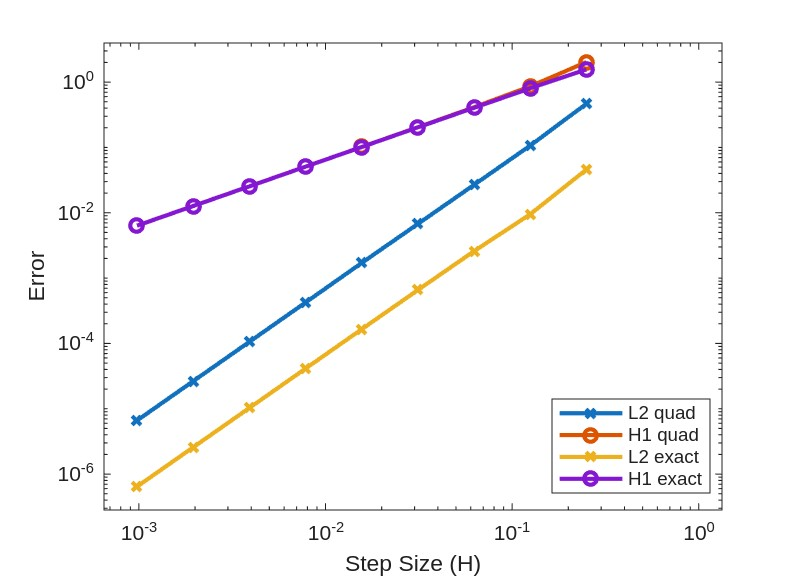
\includegraphics[width=\linewidth]{figures/dg_error_elliptic_with_and_without_quad_p1.jpg}
        \caption{Comparison of convergence rates of higher order vs lower order quadrature for $\mathcal{P}^1$-elements}
        \label{fig:elliptic_with_and_without_quad_conv_rates_p1}
    \end{minipage}
    \hfill
    \begin{minipage}[t]{0.48\textwidth}
        \centering
        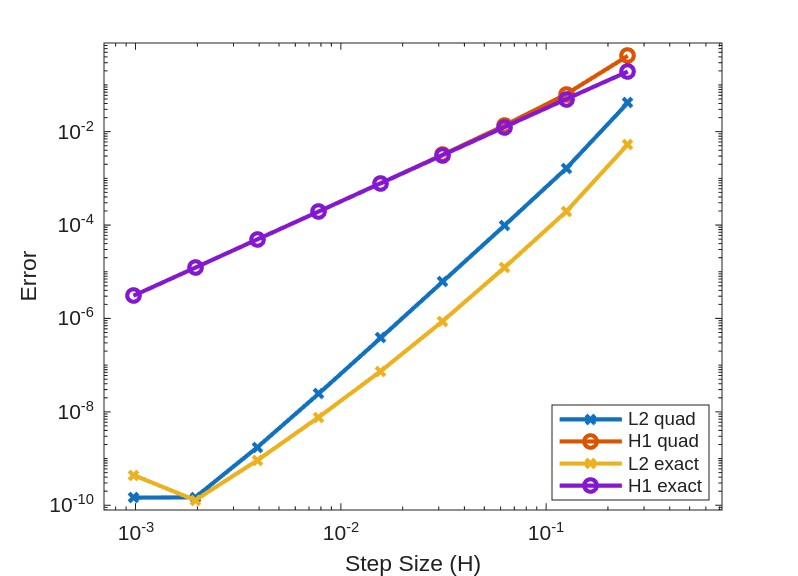
\includegraphics[width=\linewidth]{figures/dg_error_elliptic_with_and_without_quad_p2.jpg}
        \caption{Comparison of convergence rates of higher order vs lower order quadrature for $\mathcal{P}^2$-elements}
        \label{fig:elliptic_with_and_without_quad_conv_rates_p2}
    \end{minipage}
\end{figure}

\subsubsection*{Method A: "Error Quad"}
This method corresponds to exactly doing what we have been doing before. We assembled the matrices of the system (\ref{eq:elliptic_matrix_vect_system_with_mass})
as described in section \ref{sec:stiff_assembly} and approximated the integrals appearing in the entries of \textbf{A}, \textbf{M}, \textbf{l} 
using the $r+1$ node Gauss-Lobatto quadrature rule, where $r \in \{1,2\}$, meaning the quadrature nodes coincide with the basis nodes.
We calculated the $L^2, H^1(\mathcal{T}_h)$-error between the numerical solution and the exact solution on all meshes and called it \texttt{L2 quad}, \texttt{H1 quad}
respectively.

\subsubsection*{Method B: "Error Exact"}
For this method we assembled the matrices \textbf{A}, \textbf{M}, \textbf{l} for the system 
\ref{eq:elliptic_matrix_vect_system_with_mass} using $r+2$ Gauss-Lobatto quadrature nodes. This quadrature is exact for polynomials of order $2r+1$,
meaning the entries of the mass matrix \textbf{M} are calculated exactly. Next we solved the system yielding the numerical solution and in turn
calculated the $L^2, H^1(\mathcal{T}_h)$-errors on all meshes and called it \texttt{L2 exact}, \texttt{H1 exact}
respectively. 
\\ \\
In the figures \ref{fig:elliptic_with_and_without_quad_conv_rates_p1}, \ref{fig:elliptic_with_and_without_quad_conv_rates_p2} we compared 
the error rates of Method A and B and observed no significant difference but a slight downward shift of \texttt{L2 exact} on a logarithmic scale 
in comparison to \texttt{L2 quad}.